\documentclass[11pt,a4paper]{article}
    \usepackage{jinstpub}
    \usepackage{floatrow}
    \usepackage{subfig}
    \title{Quality control and batch testing for STAR-EPD front-end readout module}
    \author[a]{Liang Z.}
    \author[a]{Shen K.}
    \author[a]{Wu Y.}
    \author[a]{Shao M.}
    \affiliation[a]{University of Science and Technology of China, JinZhai Road, HEFEI, China}

    \emailAdd{liangzheng1021@163.com}
    \emailAdd{skfyl@mail.ustc.edu.cn}
    \emailAdd{torrence@mail.ustc.edu.cn}
    \emailAdd{swing@ustc.edu.cn}

    \abstract{\emph{E}vent \emph{P}lane, centrality, and trigger \emph{D}etector(EPD) is a plastic scintillation detector
    designed to be installed on RHIC-STAR. SiPMs are used to collect photons produced by scintillators, while FEE boards and RX boards are used to amplify and recieve signals from SiPMs.
    We care about their performances before installing, e.g., UI curve, noise frequency spectrum, signal characters.
    Thus, we setup a batch test system, which is made up of pulse generator, LED, digitizer, etc.
    }

    \keywords{STAR, EPD, SiPM, FEE board, RX board, Noise, Signal, Batch test}

\begin{document}
\maketitle
\flushbottom

\section{Introduction}
Relativistic Heavy Ion Collider (RHIC), locates at Brookhaven National Lab (BNL), is determined to collide heavy ions, which led to the discovery of Quark-Gluon Plasma (QGP).
The Solenoidal Tracker at RHIC (STAR) tracks particles produced by RHIC and is able to make important measurements helping answer key questions for understanding QCD matter and strong force.
The Beam Energy Scan program (BES) at RHIC has shown hints of a critical point and first-order phase transition at the BES energies.
Key measurements for locating the critical point and determining the first order phase transition are limited by poor event plane resolution, limited statistics, and a TPC-only centrality determination.
Therefore, phase II of the BES program was proposed to take data with upgraded detectors and increased statistics for the further investigation.\cite{pr17}\cite{cyang}

A new event plane and collision centrality detector is planned to replace the existing detector, the Beam-Beam Counter (BBC), with higher granularity and acceptance.
The design of the Event Plane Detector (EPD) consists of two 1.2-cm-thick plastic scintillator discs at $z= \pm 3.75~m$ from the center of STAR, covering $2.2 <\eta< 5.1$, the same as the BBC.
To maximize event plane resolution, centrality estimation and flow harmonic measurements, the disc is separated into 372 tiles (12*2 azimuthal sectors, 16+15 radial segments, see [Fig. 1]).
The emitted photons will be read out by silicon photon-multipliers (SiPM) - an inexpensive and magnetic field insensitive replacement for the traditional photo-multiplication tube, which also enhance STAR triggering capability with a nanosecond level timing resolution.

A prototype consisting of a single sector was integrated into STAR during the 2016 run and 1/8 super-sectors in 2017 run. The full EPD construction proposal was approved in 2017, while the final design was confirmed. [Refer.]
To catch up with the commissioning run in 2018 , USTC had undertook the challenging tasks for mass production and quality control of front-end readout module. which is comprised of SiPM board, front-end electronics (FEE) board, and receiver(RX) board.
Results from this first process during the construction of full EPD would be a baseline of detector performance.
In this paper, characterization of every components was researched and parameters were selected for criteria. For better efficiency and specialized operation , we developed a dedicated system for the quality control and batch test, including test platform, GUI controller, and web database. With optimized workflow and control software, we were able to achieve the extreme uniformity across all 744 channels. [JEwig-QM2018]

\section{Front-end Readout Module}
In EPD design, each channel is embedded with wavelength shifting (WLS) optical fiber wound 3 times within the tile. This is coupled to clear optical fiber which is then connected to SiPMs and finally read out by STAR FEEs/QTs.
To integrated with the STAR mechanic structure and Data Acquisition system (DAQ) [Refer], the front-end readout module of EPD is well-modularized for photo-electric conversion (SiPM), power and temperature management (FEE) as well as signal signal transmission (RX).
Considering the space of installation is rarely small, the RX board was designed as an adapter to interface between the triggering system and the FEE box ($\sim 0.5~m^3$).
For compactness, each module processes 16 channels of fiber signal, which is  attached to the SiPM board with a fiber-to-SiPM connector. [Fig. 2]

The model of SiPM for EPD is S13360-1325 from Hamamatsu. All the boards was produced and welded in professional PCB factory, while the quality control procedures are performed in out lab with specific criteria. 

\subsection{SiPM and multi-channel board}
Commercial SiPM technology has been widely used for low-photon-yield light detection in high-energy experiments. They can provide high gain ($\sim10^{6}$), high quantum efficiency ($\geq20\%$) and fast response ($\sigma_{tof}\sim250~ps$) with low voltage  ($20\sim100~V$). Since the compact structure, the signal parameters are practically independent of external magnetic fields, in contrast to standard PMT.

The multi-channel board serves as a middle-ware to aggregate all the 16 SiPMs for easy connection to the FEE board and the 3D-printer optical fiber connector. SiPM is welded on designated spot with its bias voltage and signal pin, which is linked to the gold fingers on board.[Refer] To ensure the light uniformity, upper surface of SiPMs should be almost parallel with PCB board, which means reduced variance of air gap and included angle to the fiber. For transportation safety, SiPM must be protected from dust, scratch and other possible damage by using Kapton[Refer?] and packaged in shielding bag with foam for buffering.

\subsection{FEE board}
Front-End Electronic(FEE) board is designed to communicate with computer,monitor and control bias voltage supply, amplify and output signals from SiPMs.
Connector 1 [Fig.] is for power supply, including low voltage for electronics in FEE Board and bias voltage for SiPM board; Connector 2 [Fig.] is prepared for SiPM board, which should be inserted into FEE Board; Connector 3 [Fig.] is for outputting amplified signals. Amplified signals will be sent to RX board for further digitization; Connector 4 [Fig.] is for communicating with computer. 
Bias voltage supplied to SiPM can be monitored and controlled through computer, meanwhile, current of SiPM can also be monitored. Besides, output signals’ offsets can also be adjusted through computer. Temperature compensating for bias voltage is also considered in FEE Board.
FEE Board is the most sophisticated one among the three kinds of board. Meanwhile, because its complexity, we don't have enough way to judge its functioning except by inferring from final output signal from RX board. This will be mentioned latter.

\subsection{RX board}
Due to high integration of FEE Board, there's no sufficient space for standard
connectors. Thus, Receiver(RX) Board is designed to receive signals from FEE Board and output through SMA standard connectors. RX Board is connected with FEE Board through a IEEE-1284 Compliant Parallel Cable, on which signals from SiPMs are transmitted. Then those signals will be sent to SMB connector. This will make it possible to show these signals in oscilloscope or other instruments. Detailed examination of RX board is beyond our ability. However, we can infer its
performance from its output signals. Besides, final output signals are determined by both FEE Board and RX Board, therefore, analysis of final signals can also help us judge functioning of FEE Board.
First, we concern about their noise. Lower bias voltage down to breakdown voltage of SiPMs, which is 46.1~V in our case. SiPM won't output any signal, thus, we can analyze noise of electronics. We can get noise frequency spectrum from oscilloscope in real time. Or, relatively, record several waveforms and analyze latter. Anyway, we need to ensure that the spectrum is smooth and don't have unreasonable rips.
Second, we need to measure offsets of output signals. FEE Board is able to adjust offsets in a certain range. Thus, we need to measure several offsets, under different given control parameters in computer, to get offset range and relation to control parameter.
Most importantly, we need to analyze signals from SiPMs. Although signals from SiPMs have lots of characteristics, we only concern about single photon signal. We need to see single photon peak in charge spectrum.


\section{Characterization and Quality Control}
The Quality Control (QC) process for the front-end readout module is requested to detect any device and provide a baseline of operative performance under the standards. The QC criteria have been fixed starting by the requirements to have a good uniformity between all the channels. Research on characterization was performed for helping the decision of final QC procedure and system development.

The breakdown(BD) voltage is the bias voltage at which the electric field strength generated in the depletion region is sufficient to create a Geiger discharge. It's important not only because it's what we decide working voltage on, but because it has strong relation with gain under given voltage. Two methods were used to get BD voltage, which is discussed as following.

At BD voltage point, dark current of SiPM have a rapid rise. However, after getting UI curve, different models will give different results[Refer]. This point can be measured after scaning bias voltage points and measure dark current(shown as Figure 4).
Typical UI curve of SiPM is like figure \ref{fig:ui}, which shows UI curves of all 16 SiPMs in one FEE board.
Due to low accuracy of an on-board current monitor, the precision of current measurement is less than $0.01~\mu A$.
Thus, we can only get dark current quite roughly. Despite all this, an inflection point is observed clearly when bias voltage increase.
This curve is fitted with a third order polynomial for the purpose of simplification.
At last, the point that is nearest to 0.10 $\mu A$ is appointed as operating voltage.

Gain under a certain temperature of SiPM will increase with bias voltage linearly. It's because of characteristics of quenching step. Bias voltage will decrease until no more avalanche proceeds, which means it will finally decrease to BD voltage. Thus overvoltage, which is defined as the quantity of supplied bias voltage beyond breakdown voltage, will finally decide how much
charge will be produced during avalanche. The relation is quite simple, which is $Q=C\cdot\Delta V$, where C is capacitance. Therefore, breakdown voltage can be measured from charge information of output signal.
[Fig.5a] shows a charge spectrum of SiPM under $38^{\circ}C$, measured by QDC, and deviation of two peaks shows gain of single PE. Draw gain under different bias voltage in the same graph, and use a line to fit these points, we finally get [Fig.5b]. Cross point of the line and X-axis is breakdown point, which is 51V in this case.

Gain under the same bias voltage will decrease with the increase of temperature. Higher temperature will increase concentration of charge carreier in PN knots, mean free path of which will decrease meanwhile. Thus, higer electric field strength is needed to provide enough energy for avalanching, which means breakdown voltage is higher. Finally, gain under the same bias voltage will decrease. Gain loss of temperature can be compensated by bias voltage, as is shown in [Fig].
Default compensation slope we were given is $54~mV/^{\circ}C$,which is shown in [Fig.6a]. However, gain still changes with increasing of temperature. We calculated perfect compensation slope, which is $62.5~mV/^{\circ}C$ under our circumstance, from gain-bias curve and gain-temperature curve, as is shown in [Fig.6b].

Electronic noise of these tree boards is what we concern about, because its frequency spectrum reflects electronic performance in some degree. We expect a smooth spectrum without any unreasonable rip. There are several ways to acquire the spectrum, such as oscilloscope and digitizer, and different ways gives different results. Results are discussed as below.

Many oscilloscope can replace spectrum analyzer to a certain degree, because they can do FFT in real time. However, we can record many waveforms and do FFT in computer after that. Anyway, they give the same result. However, we got unreasonable rips as figure 7a. After comparing with oscilloscope and spectrum without any input signal(figure 7b), we believe these rips are from oscilloscope and digitizer are shown in figure7a itself.

\begin{figure}[ht]
    \centering
    \subfloat[Electronic Noise by Oscilloscope]{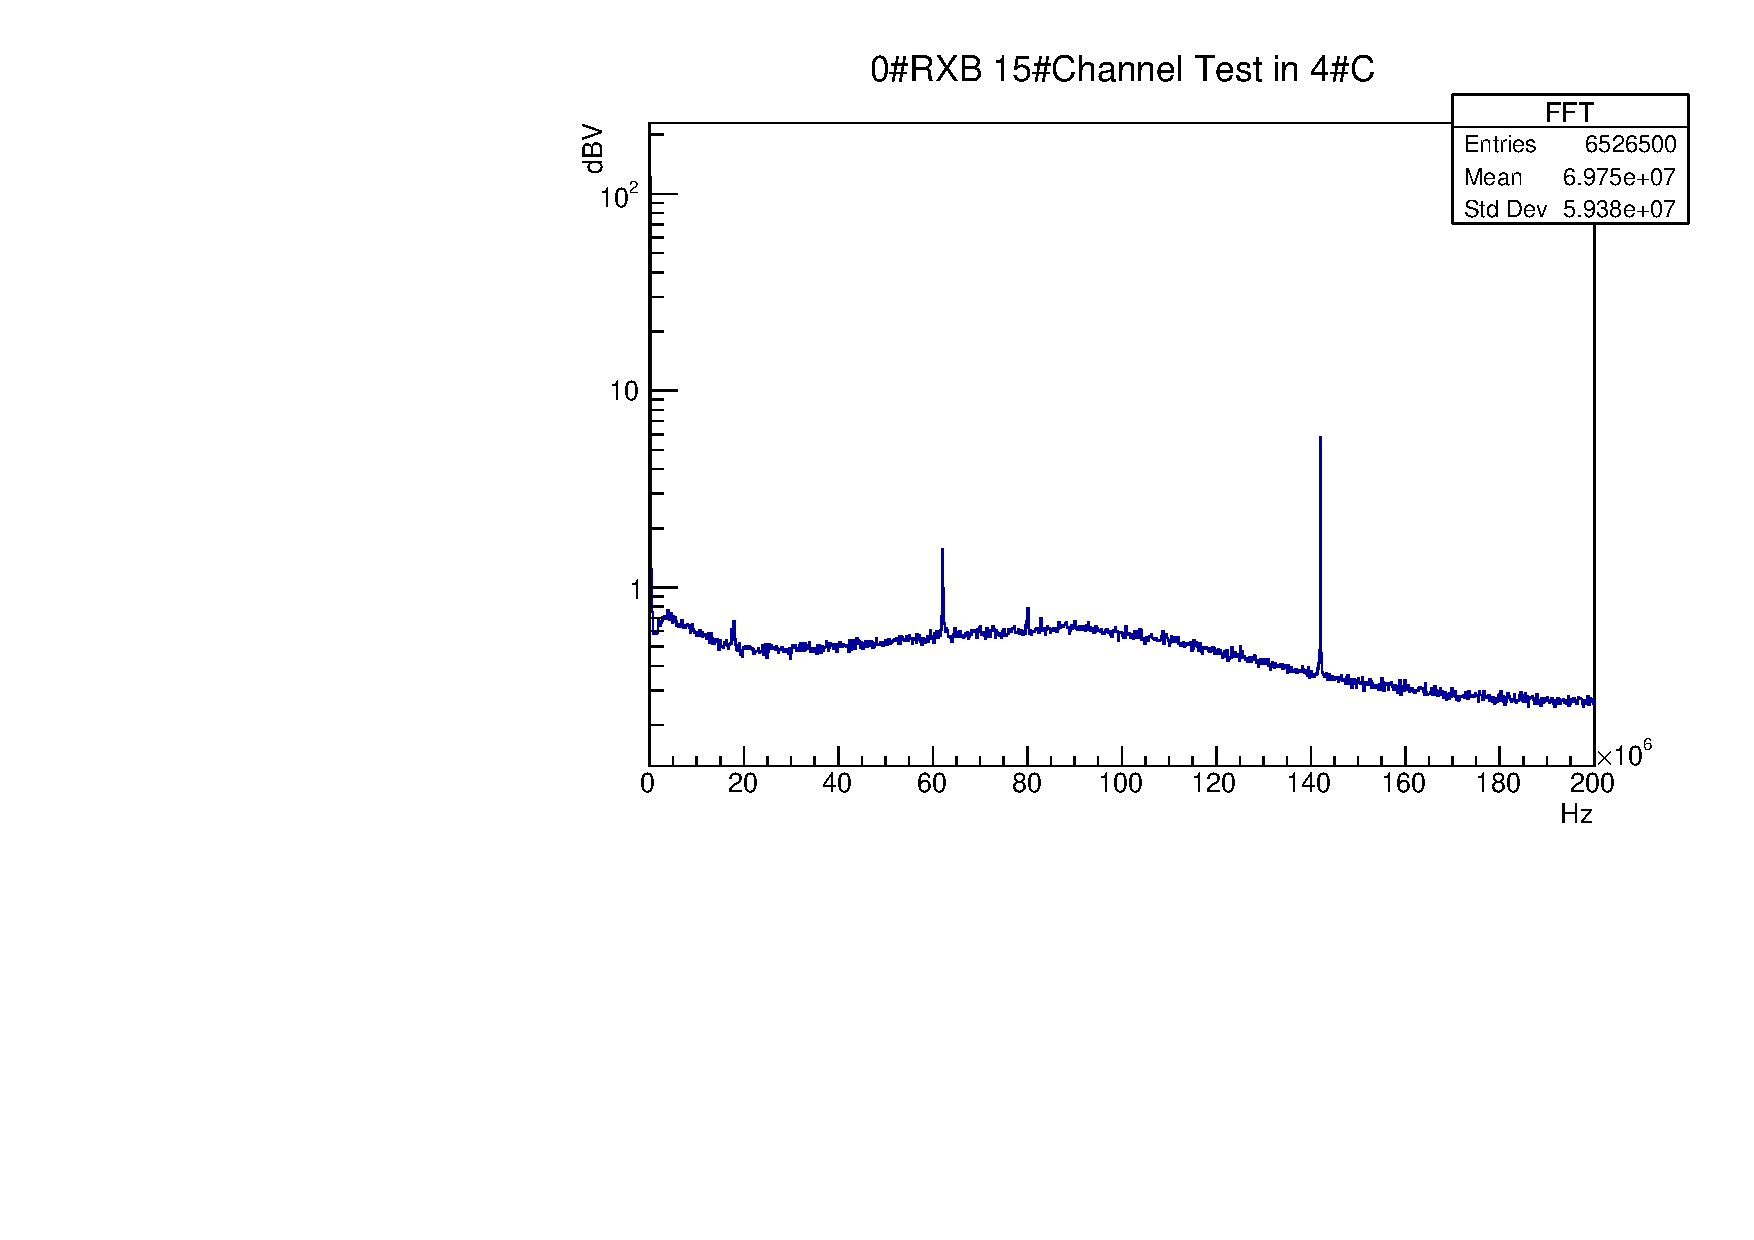
\includegraphics[width=0.45\textwidth]{fig/Noise_Osc.pdf}}\hspace{20pt}
    \subfloat[Electronic Noise by Digitizer]{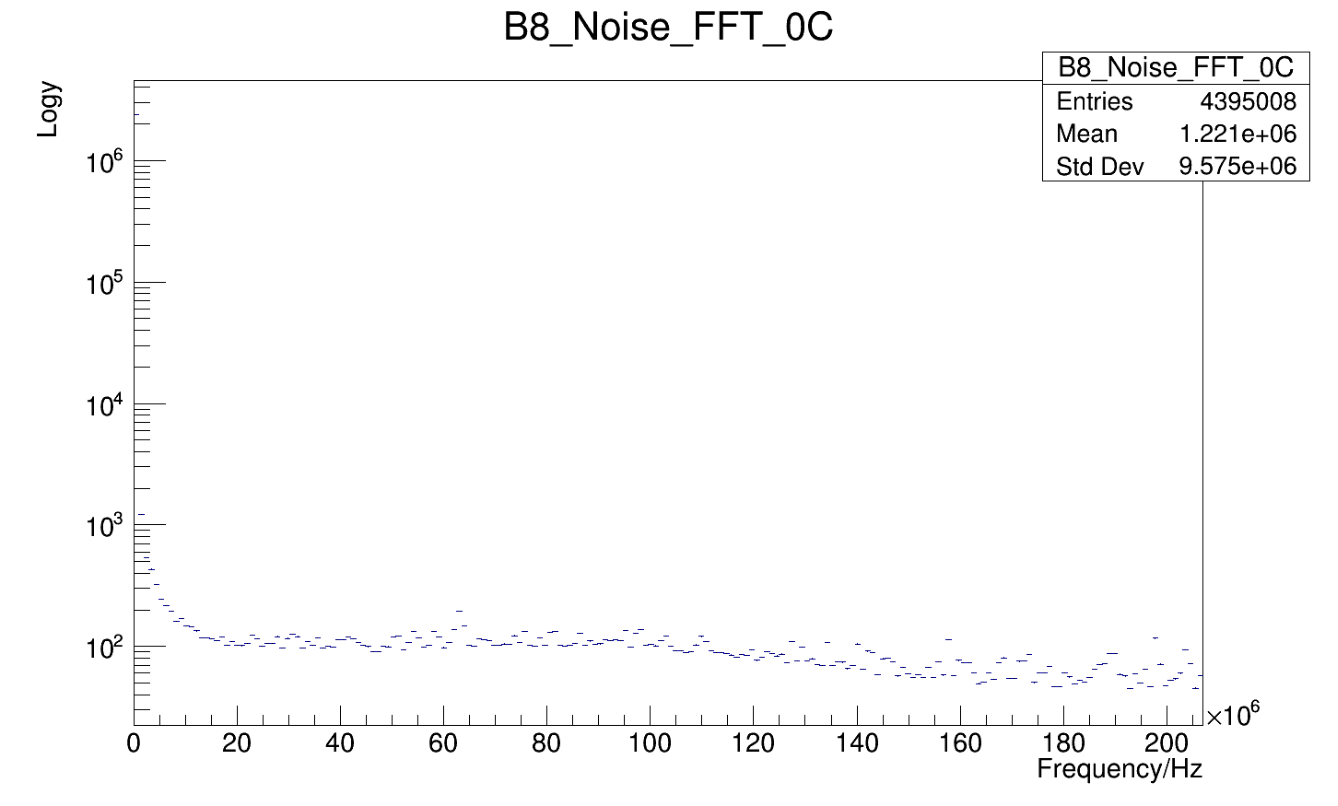
\includegraphics[width=0.45\textwidth]{fig/Noise_Dig.pdf}}\
    \subfloat[Oscilloscope Noise]{\includegraphics[width=0.45\textwidth]{fig/Osc_Noise.png}}
    % \subfloat[Digitizer Noise]{\includegraphics[scale=0.15]{_Dig_Noise.jpg}}\hspace{20pt}
    \caption{Comparison between digitizer \& oscilloscope}\label{fig:noise}
\end{figure}

It seems that results from oscilloscope are more accuracy, while results from digitizer only have a resolution of 1 MHz.
There still exist several ribs in oscilloscope noise spectrum when no signal input.
We believe it's blame to oscilloscope itself. Considering our tight schedule, we decided to use the digitizer to set up the batch test system.

Typical single photon signal is like figure8a. Obvious split of multiple photons signals can be observed. However, charge spectrum measured by QDC, like figure5a, can be used to analyze signal to noise ratio quantitatively. In addition, charge spectrum can be obtained after recording waveforms. Results from oscilloscope and digitizer are shown in figure8. Although spectrum from digitizer, in which case we use CAEN N6742, has more noise than oscilloscope, we still can seperate its multiple photons signals. Possible reasons may be poor performance of digitizer, which can be seen in figure8b. Pedestals of waveforms from digitizer are tilted, and slopes of which are different.

\paragraph{Signal}
\begin{figure}
    \centering
    % \subfloat[Signal from Oscilloscope]{
    \ffigbox[\FBwidth]{}
    {
        {
            \begin{subfloatrow}[2]
                \ffigbox[\FBwidth]{\caption{Signal from oscilloscope}}{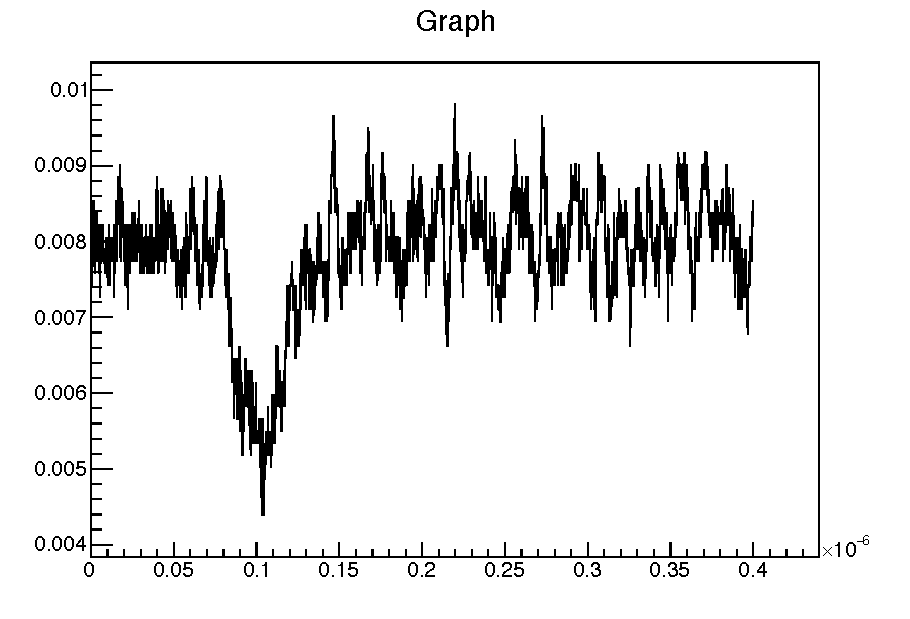
\includegraphics[scale=0.45]{fig/Signal_Osc2.pdf}}
                % \ffigbox[\FBwidth]{\caption{Signal Persistence}}{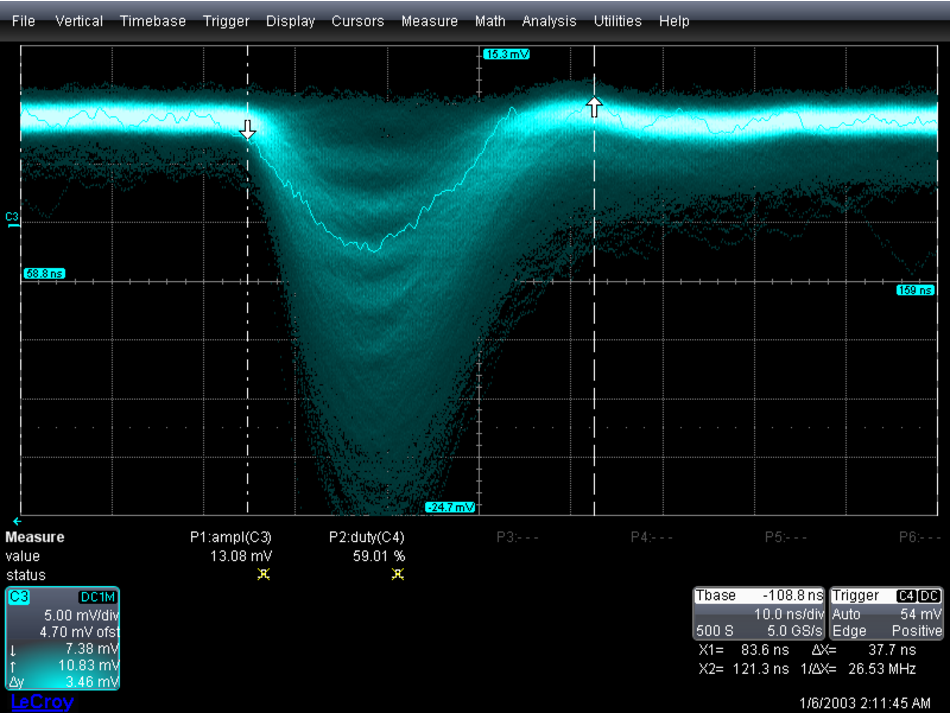
\includegraphics[scale=0.2]{Signal_Osc.pdf}}\
                \ffigbox[\FBwidth]{\caption{Signals from digitizer}\label{fig:signal-dgtz}}{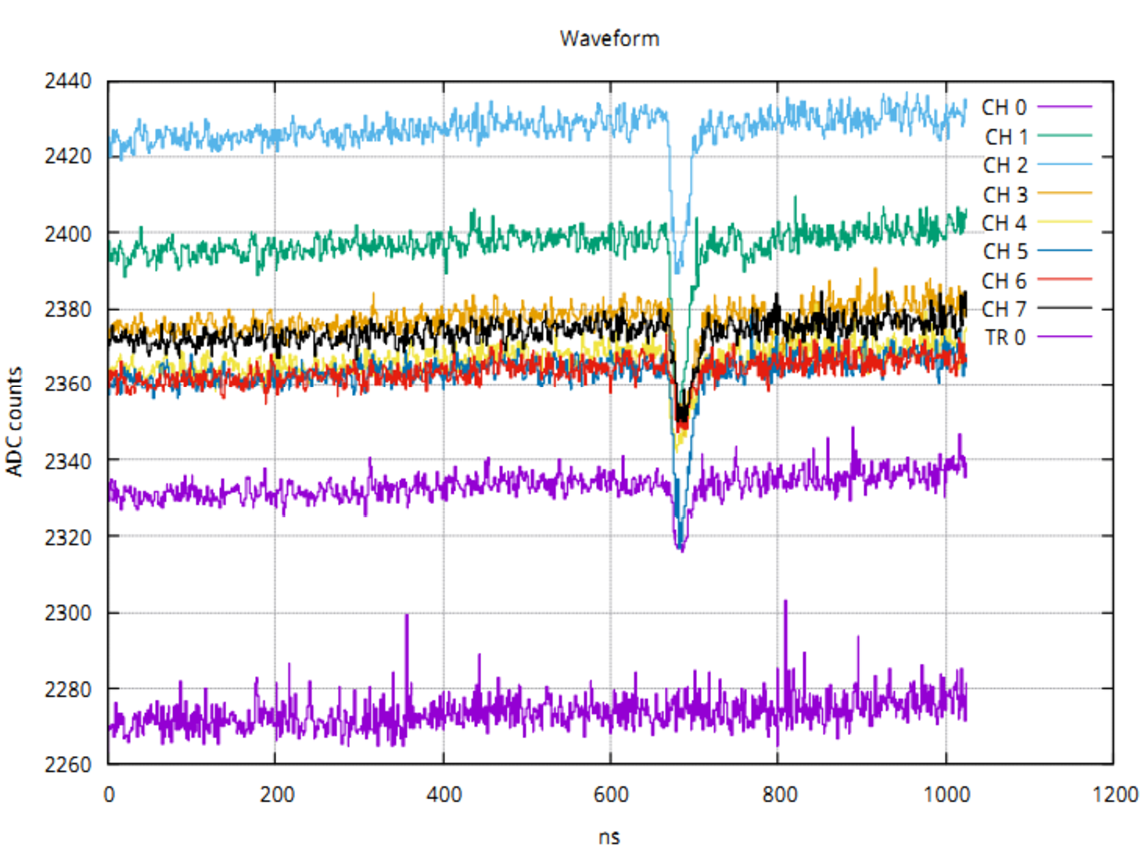
\includegraphics[scale=0.35]{fig/Signal_Dig.pdf}}
            \end{subfloatrow}
        }
        \caption{Signal Examples}\label{fig:signal}
    }
\end{figure}
Different patterns of signal samples are as shown in figure \ref{fig:signal}.

\subparagraph{Pedestal}
As is illustrated in figure \ref{fig:signal-dgtz}, pedestals of signals from digitizer are sloping.
With intensive study, this slope changes slightly when the pedestal was manipulated.
While the variance of slopes is too small to influence pedestal value, it's a reasonable convention that average value of pedestal is its measurement result.

\begin{figure}[ht]
    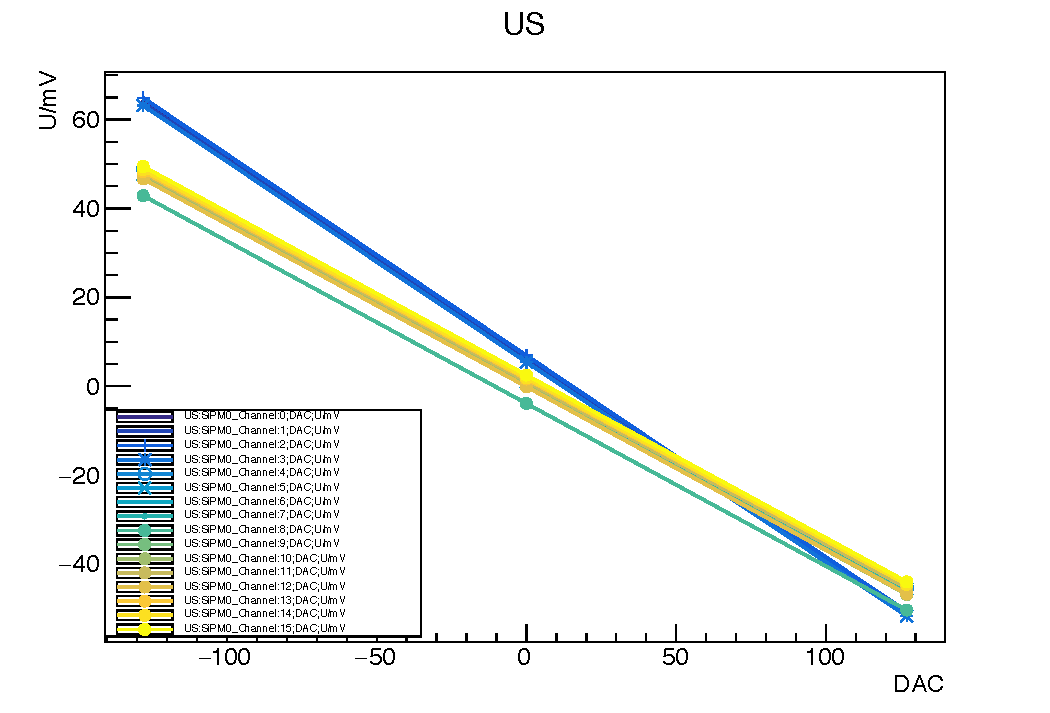
\includegraphics[scale=0.5]{fig/Pedestal.pdf}
    \caption{Pedestal Testing}\label{fig:ped}
\end{figure}

From figure \ref{fig:ped} we can see the range of pedestal for adjusting.


\subparagraph{Charge Integral of Signal}

More than 5000 signals were collected from oscilloscope/digitizer and then integrate time and amplitude. Subsequently, its spectrum was produced like figure \ref{fig:spectrum}.

There's a little trick when processing waveforms from the digitizer.
Assuming the signal interval that contains whole SiPM signals activated by photons from LED is 550ns to 650ns.
430ns to 530ns was selected as our first reference interval and 670ns to 770ns as second reference interval.
Average of this two reference intervals can be regarded as pedestal value of signal interval's midpoint.
Minusing the average value when integrating can totally get rid of the influence of pedestal slope, and improving the resolution of photon spectrum.

Furthermore, waveforms that contain the signal in reference intervals should be rejected.
It's easy to do that if we compare the slope, which is calculated by two average value of two intervals, with the distribution of slope.
If a calculated slope is far away from the mean value of pedestal distribution, this waveform should be dumped as well.
    
\begin{figure}[ht]
    \ffigbox[\FBwidth]{}{
        {
            \begin{subfloatrow}[2]
                \ffigbox{\caption{Result from oscilloscope}}{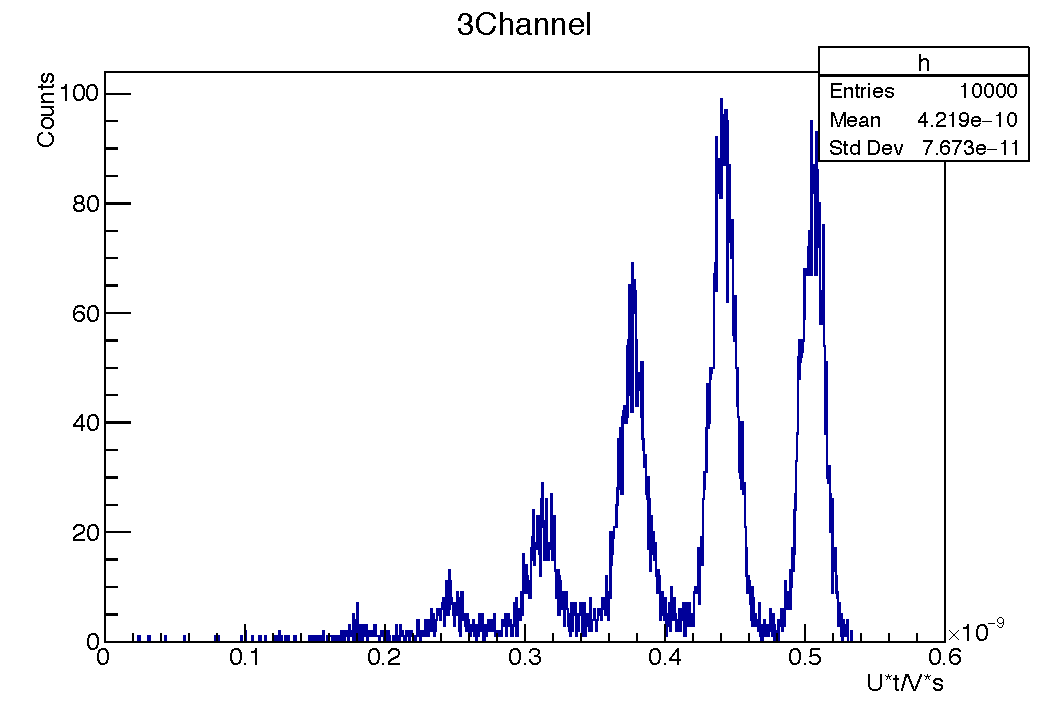
\includegraphics[width=0.45\textwidth]{fig/Oscilloscope_Integral.pdf}}
                \ffigbox{\caption{Result from digitizer}}{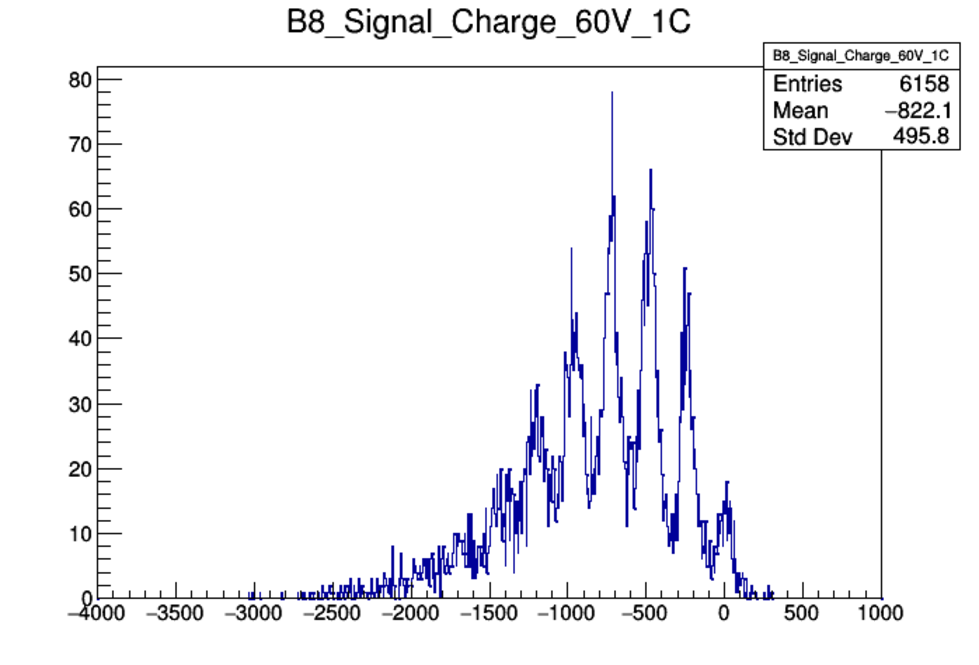
\includegraphics[width=0.45\textwidth]{fig/Digitizer_Integral.pdf}}
            \end{subfloatrow}
        }
        \caption{Integral Testing}\label{fig:spectrum}
    }
\end{figure}
    
\subsection{System Design}

Light source of the system should have the waveform that SiPM response the most. The response curve of SiPMs we use, which is Hamamatsu S13360-1325PE, is shown as figure9. Thus, we choose 470nm LED. Besides, light intensity in each channel should be as much uniform as possible. We decide to use a transparent hexagonal quartz pipe to conduct, mix and diffuse light, as is shown in figure10. LED illuminate one end of the pipe, while another end of pipe is used to cople with light fibers through a sillicon gel pad. Finally, SiPMs are illuminated by fibers at another end of fibers, between which there exists a thin air gap.

\section{System Design}
\paragraph{Test Items \& Test Methods}First, all device's mechanical integrity should be ensured and SiPMs' thickness should be measured,
i.e., we should first check whether there exists any obvious damage and than measure thickness of SiPM by microscope.

Second, UI curve of a SiPM can help us judge its basic electric properties, e.g., dark current and break down(BD) voltage.
Under good dark conditions, we change bias voltage on SiPMs from 50V to 65V, with 0.5V step size. This range covers all what we are interested in.
We can control FEE board and acquire U/I information through computer.

Third, electronic noise can reflect electronic performances. Rib or strange peaks shouldn't appear in noise frequency spectrum. Thus, we set bias voltage on
SiPM at 46.5V, which is below its BD voltage, and output RX board signal into oscilloscope or digitizer to collect waveforms, and finally get frequency spectrum.

Last, several characters of SiPM's signal should be tested. Shape of signal should be normal, and pedestal should be changed when adjusting DAC. In addition, we need check
spectrum of signal charge integral in order to judge the quality of single photon signal's resolution. We first set bias voltage below BD voltage(46.5V) to check pedestal. And
then, set bias voltage at OP voltage(60V) to check integral spectrum, meanwhile, illuminate SiPMs with light from a LED, which is driven by wavefrom generator. Output all signal
into oscilloscope/digitizer, which is triggered in the same frequency as LED. After collecting enough waveforms and a little further processing, we get integral spectrum.

\paragraph{System Chart}
System chart is as shown in figure \ref{fig:System Chart}.

\paragraph{Instrument Selection}It's easy to choose LED, whose luminous wavelength range should cover peak of scintillators' luminescence spectrum, i.e., 475nm.
However, choosing oscilloscope or digitizer is a tough decision. Oscilloscope can help to get more accurate result, but only have 4 input channels. While digitizer have
16 channels but has less precision. Besides, digitizer should be calibrated before using.

\begin{figure}[ht]
    \centering
    \begin{floatrow}
        \centering
        \ffigbox{\caption{System Chart}\label{fig:System Chart}}{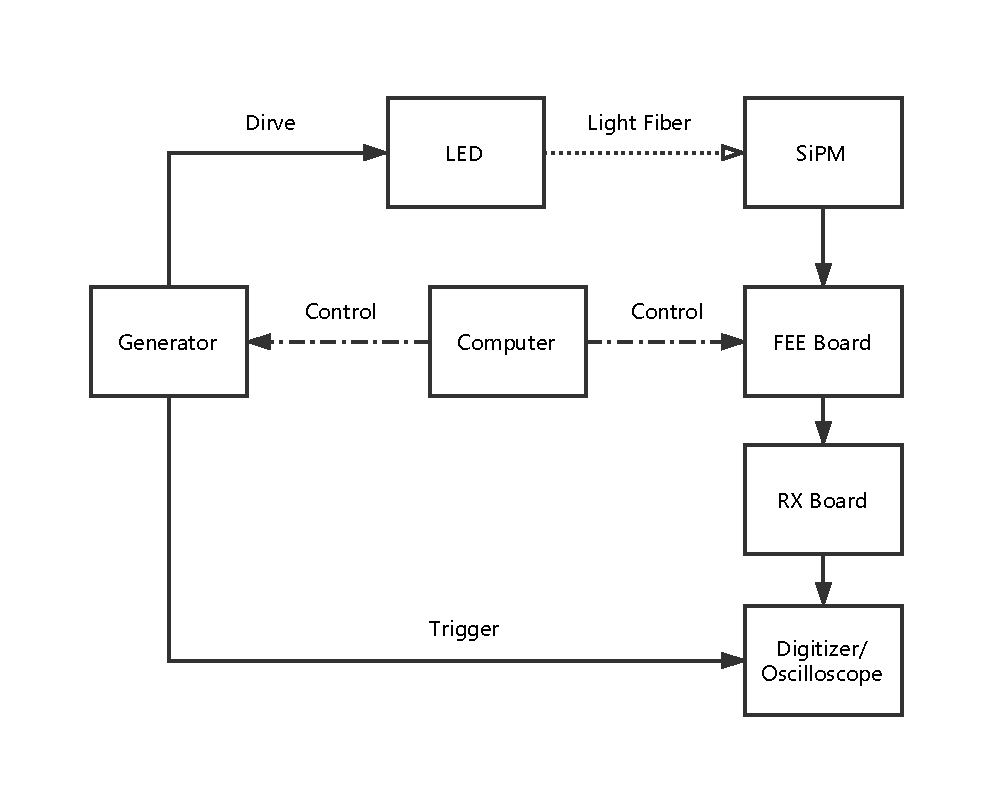
\includegraphics[scale=0.45]{fig/System_Chart.pdf}}
        \centering
        \ffigbox{\caption{UI Curve Example}\label{fig:UI Curve Example}}{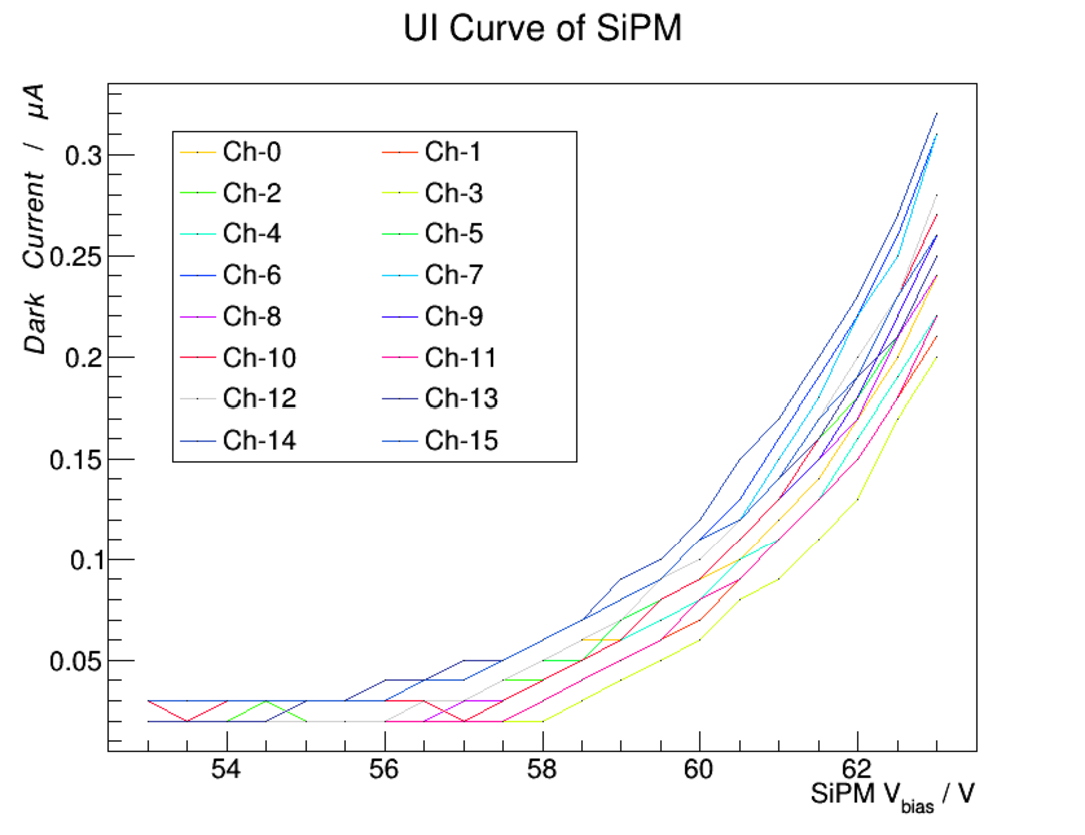
\includegraphics[scale=0.4]{fig/UI_Curve.pdf}}

    \end{floatrow}
    % \includegraphics[scale=0.25]{Flow_Chart.png}
\end{figure}




\section{Batch Test}
% \paragraph{Digitizer Calibration}Due to tight time schedule, we decide to use digitizer instead of oscilloscope.
% However, calibration of digitizer should be done before we setup batch test system.
% Have pulse generator generated pulses with different amplitudes. And output them seperately to digitizer and oscilloscope.
\section{Summary}
% \subsection{}


\end{document}
